\chapter{Experimentación y resultados}
\label{cap:experimentacion}

El presente capítulo expone de forma pormenorizada la fase de validación empírica y el análisis de resultados de las arquitecturas neuronales implementadas. Atendiendo a los objetivos de la investigación, la experimentación se diseña para validar la eficacia matemática de los modelos frente a dinámicas complejas del tráfico urbano. A lo largo de las siguientes secciones, se detallan las restricciones operativas del entorno, se analiza la convergencia de los modelos durante la fase de entrenamiento y se exponen las métricas obtenidas sobre el conjunto de datos inexplorado (\textit{test}).





\section{Restricciones experimentales}
\label{sec:experimental_design}

Previamente al análisis cuantitativo de los resultados, se definen ciertas consideraciones y restricciones de \textit{hardware} que han moldeado la ejecución de los experimentos. La optimización de arquitecturas de \textit{Deep Learning} sobre series temporales multivariantes exige establecer un balance realista entre el rigor metodológico teórico y la viabilidad computacional.

\subsection{Restricciones en la exploración paramétrica para CSDI}

Como se ha definido anteriormente en el diseño arquitectónico, el sistema implementa una búsqueda aleatoria probabilística configurada a 22 iteraciones para garantizar un intervalo de confianza estadístico superior al 90\% en el hallazgo de hiperparámetros óptimos. Sin embargo, cabe destacar una excepción a esta premisa teórica debido al extremo coste temporal observado durante el entrenamiento del modelo de imputación CSDI. Al tener que realizarse una inversión del ruido estocástico a través de cadenas de Márkov, la ejecución de 22 iteraciones no es asumible con la infraestructura computacional disponible. En consecuencia, la exploración para CSDI se limita a 8 pruebas, lo cual supone un \textit{trade-off} importante: se reduce significativamente la probabilidad de obtener la mejor configuración en favor de viabilizar la ejecución del experimento en tiempos razonables.

\subsection{Ajuste de tamaño de ventana para MICN}

En los experimentos de predicción es necesario establecer una relación coherente entre el tamaño de ventana de observación histórica ($L_{in}$) y el horizonte de predicción objetivo ($L_{out}$). Para los escenarios a corto plazo (predicción a 24 horas), se establece que la ventana de entrada es del doble de tamaño que el horizonte temporal. Dado un muestreo de 15 minutos ($L_{out}^{24h}=96$ pasos), la entrada se configura con 192 pasos ($L_{in}^{24h}=192$). Esta configuración proporciona al modelo información suficiente para capturar patrones diarios completos y ha sido utilizada de forma consistente en todas las arquitecturas evaluadas, a excepción de MICN.

Para el escenario de predicción a 48 horas ($L_{out}^{48h}=192$ pasos), mantener la misma relación implica utilizar una ventana de entrada de 384 pasos ($L_{in}^{48h}=384$). Sin embargo, durante las pruebas preliminares realizadas con la implementación de MICN de PyPOTS, esta configuración ha producido errores internos asociados a las operaciones convolucionales del modelo. Concretamente, tras las etapas de submuestreo y transformación multiescala, algunas capas convolucionales internas han intentado aplicar filtros de tamaño superior a la longitud efectiva de la secuencia procesada, colapsando la red.

Cabe destacar que el problema no se ha observado en configuraciones con $L_{in}=192$, tanto para horizontes de 96 como de 192 pasos, lo que sugiere una limitación práctica de la implementación utilizada para determinadas combinaciones de ventana de entrada y horizonte de predicción, más que una limitación inherente a la arquitectura MICN.

Por este motivo, para el escenario de predicción a 48 horas se opta por adoptar una configuración con ventana de entrada igual al horizonte de predicción ($L_{in}^{48h}=L_{out}^{48h}=192$) para garantizar estabilidad durante el entrenamiento.





\section{Análisis del Entrenamiento y Validación}
\label{sec:training_validation_results}

Antes de someter las arquitecturas al conjunto de \textit{test}, resulta imprescindible auditar la fase de entrenamiento y el proceso de optimización de hiperparámetros (HPO). El objetivo de esta fase metodológica es identificar la configuración estructural que maximice la capacidad de generalización de cada modelo, utilizando el MAE sobre el conjunto de validación como métrica objetivo.

La Tabla \ref{tab:resultados_validacion} consolida las métricas de error alcanzadas en validación por las configuraciones óptimas que resultan seleccionadas para la evaluación final.

\begin{table}[H]
	\centering
	\caption{MAE alcanzado en el conjunto de validación tras la búsqueda de hiperparámetros.}
	\label{tab:resultados_validacion}
	\begin{tabular}{llc}
		\toprule
		\textbf{Tarea / Horizonte} & \textbf{Modelo} & \textbf{MAE (Validación)} \\
		\midrule
		\multirow{2}{*}{\textbf{Imputación}} & SAITS & 0.04961 \\
		& CSDI & 3.84810 \\
		\midrule
		\multirow{3}{*}{\textbf{Predicción (24 Horas)}} & MICN & 0.03914 \\
		& DLinear & 0.06295 \\
		& Transformer & 0.25028 \\
		\midrule
		\multirow{3}{*}{\textbf{Predicción (48 Horas)}} & MICN & 0.04536 \\
		& DLinear & 0.06060 \\
		& Transformer & 0.29357 \\
		\bottomrule
	\end{tabular}
\end{table}

Para indagar en las discrepancias de rendimiento expuestas en la tabla anterior, resulta indispensable auditar el comportamiento dinámico de las redes durante la fase de aprendizaje. La telemetría extraída de TensorBoard permite analizar las curvas de convergencia y diagnosticar las limitaciones subyacentes de cada topología.

\subsection{Análisis de convergencia en modelos de imputación}

El rendimiento anómalo de CSDI requiere un análisis visual detallado de sus curvas de aprendizaje.

\begin{figure}[htbp]
	\centering
	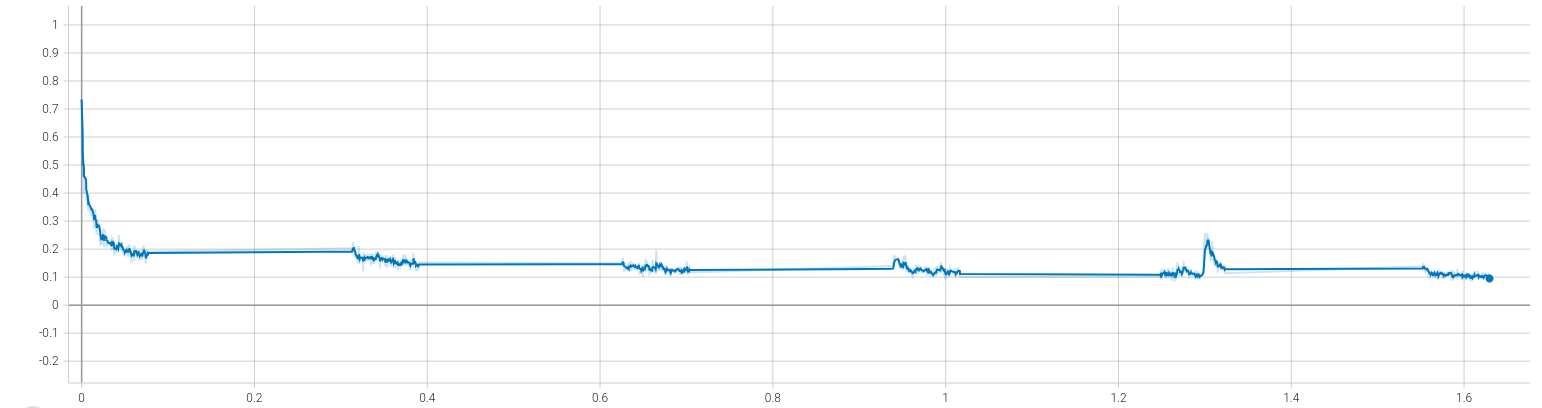
\includegraphics[width=0.48\textwidth]{img/[exp]csdi_tl.png}
	\hfill
	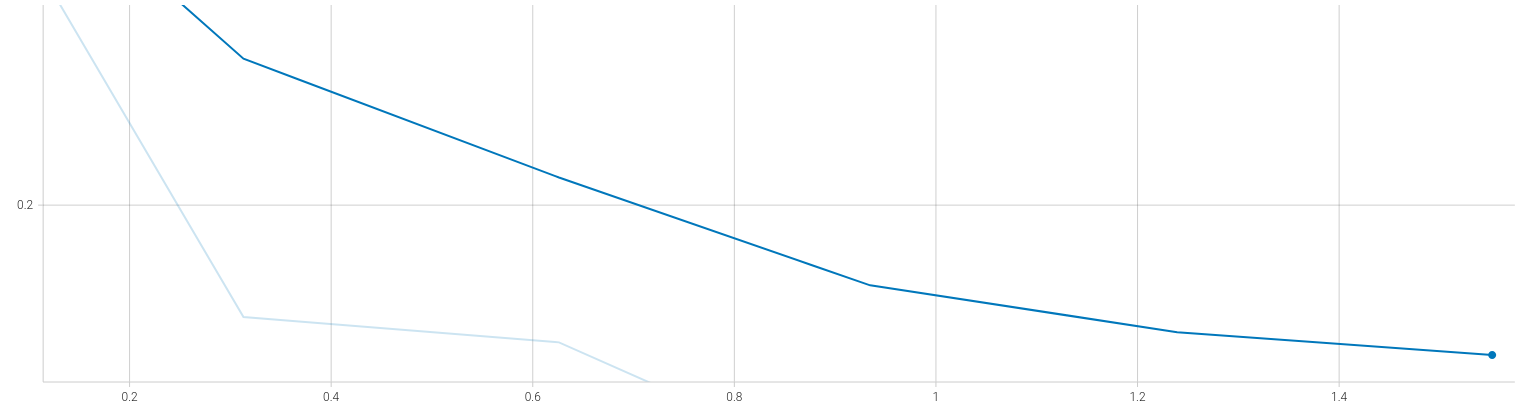
\includegraphics[width=0.48\textwidth]{img/[exp]csdi_vl.png}
	\caption{Curvas de convergencia para el modelo CSDI. Izquierda: evolución de la función de pérdida en entrenamiento. Derecha: función de pérdida en validación.}
	\label{fig:tensorboard_csdi}
\end{figure}

Al observar la Figura \ref{fig:tensorboard_csdi}, la curva de entrenamiento muestra un descenso precipitado inicial seguido de un estancamiento prolongado. En CSDI, la función de pérdida mostrada en la gráfica no representa el MAE directo de la serie temporal, sino el error de estimación del ruido residual ($\epsilon$-matching) inyectado durante la cadena de Márkov. El modelo logra aprender a eliminar ruido gaussiano genérico con relativa rapidez, pero es incapaz de reconstruir la distribución real del tráfico urbano.

Como se documenta en la literatura especializada sobre difusión generativa \parencite{ho2020denoising}, estas arquitecturas resultan extremadamente demandantes en términos de volumen de datos y ciclos de ajuste. La dificultad que enfrenta el modelo probabilístico para mapear el espacio latente multivariante con precisión no se atribuye exclusivamente a la limitación de la búsqueda paramétrica, sino también al establecimiento de un máximo de 20 épocas y a la insuficiencia de la longitud de los datos de entrenamiento para este tipo de arquitecturas.

\subsection{Análisis de convergencia en modelos de predicción}

En el dominio de \textit{forecasting}, los resultados de la Tabla \ref{tab:resultados_validacion} revelan una marcada superioridad de las arquitecturas MICN y DLinear frente al modelo basado en autoatención. Para justificar matemáticamente esta divergencia, resulta de gran utilidad contrastar de forma directa sus curvas de convergencia durante la fase de entrenamiento, ilustradas en la Figura \ref{fig:tensorboard_forecasting}.

\begin{figure}[htbp]
	\centering
	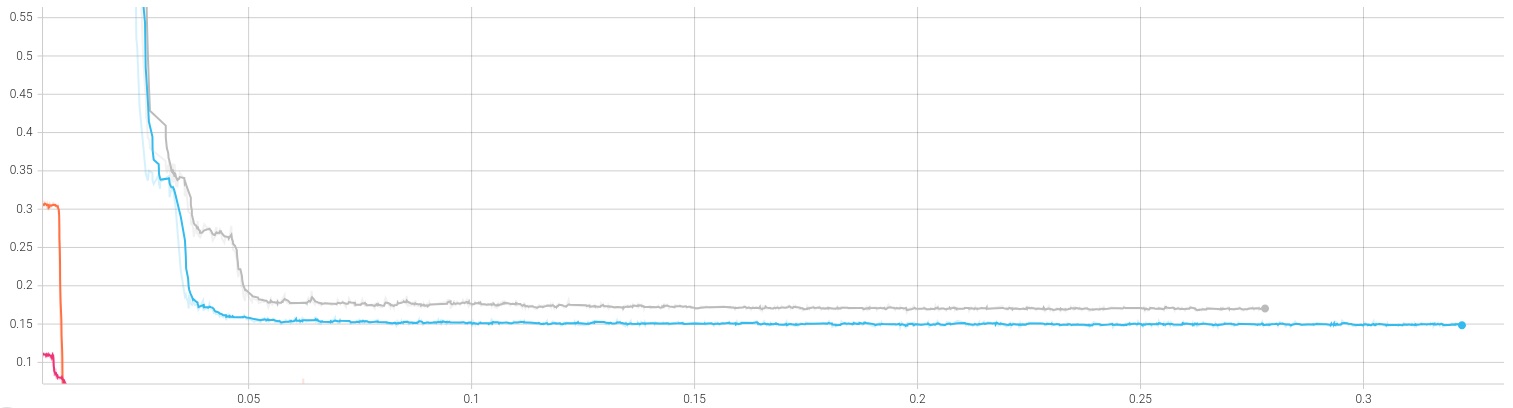
\includegraphics[width=0.9\textwidth]{img/[exp]micn_transf_tl.png}
	\caption{Comparativa de la función de pérdida en entrenamiento entre MICN (naranja y rosado) y Transformer (azul y gris) para ambos horizontes predictivos.}
	\label{fig:tensorboard_forecasting}
\end{figure}

El registro visual proporciona una confirmación empírica rotunda de la eficiencia computacional de las redes convolucionales frente a los mecanismos de atención puros en series temporales continuas. Al analizar la telemetría de MICN, se observa un desplome casi vertical del error durante los primeros compases del entrenamiento. La función de pérdida desciende rápidamente y se estabiliza de inmediato en valores próximos a cero: las convoluciones locales para alta frecuencia y las isométricas para tendencias globales extraen exitosamente las dinámicas del tráfico urbano.

En contraste, las trazas correspondientes a las ejecuciones del Transformer muestran una dinámica de aprendizaje mucho más ineficiente. El modelo inicia su ajuste con magnitudes de error significativamente mayores, y, aunque experimenta un descenso inicial pronunciado, esta caída deriva en un estancamiento prolongado que la red neuronal es incapaz de perforar (rango aproximado de 0.15 - 0.20). La causa estructural de este comportamiento se encuentra documentada en la literatura reciente. Como argumentan \textcite{zeng2023are}, el mecanismo de autoatención puro es inherentemente invariante a las permutaciones. Aunque esta limitación teórica se mitiga mediante codificaciones posicionales (\textit{positional encodings}), en el dominio de las series temporales numéricas y continuas esta estrategia resulta subóptima. El modelo atencional tiende a priorizar el cálculo de similitudes semánticas punto a punto, lo que provoca una pérdida de información sobre el orden cronológico estricto y limita su capacidad para abstraer la macrotendencia frente a enfoques puramente lineales o convolucionales.





\section{Resultados en Tareas de Imputación}
\label{sec:results_imputation}

Una vez aisladas y validadas las mejores configuraciones arquitectónicas, se evalúan los modelos neuronales SAITS y CSDI, así como los estimadores estadísticos de referencia (Media Global y LOCF) en el mismo conjunto de datos inexplorado de \textit{test}. Los resultados obtenidos tras el proceso de inferencia se detallan en la siguiente tabla de métricas:

\begin{table}[H]
	\centering
	\caption{Métricas de evaluación en el conjunto de test para tareas de imputación.}
	\label{tab:resultados_imputacion}
	\begin{tabular}{lccc}
		\toprule
		\textbf{Modelo / Algoritmo} & \textbf{MAE} & \textbf{MSE} & \textbf{RMSE} \\
		\midrule
		\textbf{SAITS} & \textbf{0.05555} & \textbf{0.01189} & \textbf{0.10902} \\
		Media Global & 0.37965 & 0.26472 & 0.51451 \\
		LOCF & 0.53709 & 61.99049 & 7.87340 \\
		CSDI & 3.83389 & 100.37682 & 10.01882 \\
		\bottomrule
	\end{tabular}
\end{table}

El análisis de las métricas arroja conclusiones determinantes sobre la reconstrucción de la señal:

\begin{enumerate}
	\item \textbf{El colapso del algoritmo de inercia (LOCF).}
	Aunque su Error Absoluto Medio (0.537) es deficiente pero acotado, su Error Cuadrático Medio se dispara de forma anómala (MSE de 61.99). Este fenómeno posee una explicación matemática fundamentada en la naturaleza del sensor: la ocupación de estacionamiento experimenta cambios de estado binarios o muy abruptos (por ejemplo, cuando un vehículo abandona la plaza). Si un sensor queda inactivo tras registrar un estado de alta ocupación, el algoritmo LOCF propaga ese estado de forma estática durante horas. Al elevar al cuadrado la diferencia acumulada frente a la realidad dinámica, la penalización escala masivamente, lo que demuestra empíricamente que la inercia temporal no es una heurística válida para entornos de movilidad volátiles.
	
	\item \textbf{La superioridad determinista de SAITS.}
	La arquitectura SAITS domina la comparativa de forma absoluta: obtiene un MAE de 0.055 que ratifica la solidez de lo aprendido en validación. Al impedir que el modelo observe la coordenada exacta que debe predecir mediante el enmascaramiento diagonal, la red se ve forzada a asimilar la estacionalidad periódica extraída de los pasos adyacentes. Su bajísimo RMSE (0.109) confirma la práctica ausencia de \textit{outliers} en su reconstrucción.
	
	\item \textbf{La divergencia de CSDI.}
	El rendimiento de la arquitectura CSDI en el conjunto inexplorado (MAE de 3.833) es prácticamente diez veces superior al de un promedio simple como la Media Global. Como se aborda en la Sección \ref{sec:experimental_design}, las severas restricciones computacionales merman el potencial de la arquitectura probabilística generativa.
\end{enumerate}






\section{Resultados en Tareas de Predicción}
\label{sec:results_forecasting}

Por otro lado, se evalúa la capacidad de proyección futura de las arquitecturas neuronales en dos horizontes: a corto plazo (24 horas) y a medio plazo (48 horas). Las métricas arrojadas por la evaluación en el conjunto de prueba se consolidan en la siguiente comparativa:

\begin{table}[H]
	\centering
	\caption{Métricas de evaluación en el conjunto de test para tareas de predicción a 24 y 48 horas.}
	\label{tab:resultados_forecasting}
	\begin{tabular}{llccc}
		\toprule
		\textbf{Horizonte} & \textbf{Modelo} & \textbf{MAE} & \textbf{MSE} & \textbf{RMSE} \\
		\midrule
		\multirow{3}{*}{\textbf{24 Horas}} & \textbf{MICN} & \textbf{0.03848} & 0.02181 & 0.14768 \\
		& DLinear & 0.06503 & \textbf{0.02013} & \textbf{0.14188} \\
		& Transformer & 0.26443 & 0.15471 & 0.39334 \\
		\midrule
		\multirow{3}{*}{\textbf{48 Horas}} & \textbf{MICN} & \textbf{0.04639} & 0.02492 & 0.15787 \\
		& DLinear & 0.07342 & \textbf{0.02136} & \textbf{0.14615} \\
		& Transformer & 0.30828 & 0.17860 & 0.42261 \\
		\bottomrule
	\end{tabular}
\end{table}

El comportamiento predictivo de las redes neuronales se desglosa a continuación:

\begin{enumerate}
	\item \textbf{La confirmación empírica del fracaso atencional puro.}
	Los resultados validan concluyentemente la tesis expuesta en el marco teórico respecto a las limitaciones topológicas del Transformer \parencite{zeng2023are}. La arquitectura Transformer se sitúa como la más ineficiente en ambos escenarios. 
	
	\item \textbf{La similitud de rendimiento entre la convolución isométrica y la descomposición lineal.}
	La comparativa entre MICN y DLinear aporta el análisis empírico más interesante de la experimentación. \textbf{MICN se consolida como el modelo más preciso en términos de error absoluto} para ambos horizontes temporales. Su doble convolución estructural modela con enorme agudeza la volatilidad urbana diaria. Sin embargo, \textbf{DLinear obtiene los mejores registros en la minimización del error cuadrático} (MSE de 0.020 y 0.021). Al proyectar matemáticamente tendencias mediante capas densas directas, DLinear asume un comportamiento conservador: evita predecir anomalías extremas, lo que le otorga gran inmunidad frente a las penalizaciones del MSE, a expensas de sacrificar precisión fina.
	
	\item \textbf{La resiliencia al aumentar el horizonte temporal.}
	Escalar el horizonte predictivo revela la solidez de la aproximación paramétrica, cuyo MAE apenas experimenta degradación de 0.065 a 0.073. Por su parte, la arquitectura MICN muestra una caída predecible puesto que procesa la mitad del contexto histórico. Aun así, alcanza el mejor MAE.
\end{enumerate}





\section{Evaluación Compuesta del Pipeline Predictivo}
\label{sec:pipeline_results}

Como culminación de la fase de experimentación, se ejecuta el flujo algorítmico integrado que incluye los dos subdominios de la investigación. El propósito de este ensayo empírico consiste en cuantificar si las arquitecturas de predicción experimentan una mejora significativa en su rendimiento al recibir un contexto histórico reconstruido previamente por SAITS (sin valores faltantes), frente a procesar directamente la señal cruda con los vacíos naturales de los sensores.

Para garantizar la rigurosidad del análisis, se seleccionan cuatro escenarios de prueba estratégicos con diferentes combinaciones de modelos y horizontes temporales. Los resultados obtenidos de someter el mismo conjunto de prueba a las redes de predicción de forma aislada y, posteriormente, a través del \textit{pipeline} de preprocesamiento con SAITS, se consolidan en la Tabla \ref{tab:resultados_pipeline}.

\begin{table}[H]
	\centering
	\caption{Resultados del \textit{pipeline} integrado. Comparativa de error MAE sobre datos originales frente a datos previamente imputados por SAITS.}
	\label{tab:resultados_pipeline}
	\begin{tabular}{llccc}
		\toprule
		\textbf{Pipeline (Imputador $\rightarrow$ Predictor)} & \textbf{Estado} & \textbf{MAE} & \textbf{MSE} & \textbf{Var. (\%)} \\
		\midrule
		\multirow{2}{*}{SAITS $\rightarrow$ \textbf{MICN (24H)}} 
		& Crudo & 0.03845 & 0.02177 & \multirow{2}{*}{\textcolor{green!70!black}{-0.05\%}} \\
		& Imputado & \textbf{0.03843} & \textbf{0.02165} & \\
		\midrule
		\multirow{2}{*}{SAITS $\rightarrow$ \textbf{DLinear (24H)}} 
		& Crudo & 0.06503 & 0.02010 & \multirow{2}{*}{\textcolor{green!70!black}{-0.49\%}} \\
		& Imputado & \textbf{0.06471} & \textbf{0.02006} & \\
		\midrule
		\multirow{2}{*}{SAITS $\rightarrow$ \textbf{DLinear (48H)}} 
		& Crudo & \textbf{0.07342} & \textbf{0.02136} & \multirow{2}{*}{\textcolor{red!70!black}{+0.49\%}} \\
		& Imputado & 0.07378 & 0.02136 & \\
		\midrule
		\multirow{2}{*}{SAITS $\rightarrow$ \textbf{Transformer (24H)}} 
		& Crudo & 0.26451 & 0.15475 & \multirow{2}{*}{\textcolor{green!70!black}{-0.04\%}} \\
		& Imputado & \textbf{0.26440} & \textbf{0.15473} & \\
		\bottomrule
	\end{tabular}
\end{table}

Tras analizar los resultados obtenidos y ponderar los costes computacionales asociados, se concluye lo siguiente:

\begin{enumerate}
	\item \textbf{El SOTA es robusto por naturaleza.}
	El primer escenario evalúa la sinergia entre dos modelos con alta precisión como son SAITS y MICN. En un inicio, es posible creer que si MICN exhibe un rendimiento sobresaliente asimilando datos con ruido, una señal bien imputada debería acercar el error a un mínimo teórico. Sin embargo, los resultados demuestran que la mejora es virtualmente inexistente, con una reducción del 0.05\% en el error. Un fenómeno idéntico se observa al purificar la entrada de DLinear a 24 horas.
	
	Este hallazgo es crucial: ambos modelos de \textit{forecasting} actúan como mecanismos de suavizado resilientes para los valores nulos. La arquitectura interna de estos modelos asimila las anomalías de los sensores con tal eficacia que anula la necesidad de aplicar técnicas generativas de imputación previas.
	
	\item \textbf{La propagación de error por escalabilidad.}
	Al someter el flujo a un escenario de alta exigencia (SAITS acoplado a DLinear con ventana histórica de 384 pasos), la imputación degrada ligeramente el rendimiento. Se observa el problema clásico de la propagación del error en inferencias en cascada: la reconstrucción de SAITS es muy precisa, aunque introduce pequeñas desviaciones sobre los vacíos del sensor, que en una ventana tan dilatada hacen que la señal acumule un sesgo sintético notable. Consecuentemente, se confunde ligeramente a la capa lineal del modelo predictivo, lo cual resulta más perjudicial que omitir el dato faltante original.
	
	\item \textbf{La refutación algorítmica del Transformer:}
	Dado el rendimiento deficiente del Transformer sobre la señal original, se ha buscado determinar si su colapso obedece a una escasa tolerancia a los valores ausentes o a una deficiencia topológica profunda. Al inyectar la señal reconstruida, se observa que la mejora en el error predictivo es estadísticamente nula: se ratifica la hipótesis previamente planteada para el Transformer.
\end{enumerate}




\section{Evaluación sobre el \textit{dataset Out-Of-Time}}
\label{sec:results_oot}

Una vez se ha probado la correcta ejecución de los modelos en el conjunto histórico, es importante probar que estas tengan capacidad para generalizar en un entorno de producción. Por consiguiente, todos los modelos seleccionados se someten a una fase de evaluación sobre un subconjunto (por limitaciones de GPU) del dataset de datos adquirido en tiempo real durante el mes de mayo. Al alimentar las redes con datos de un mes en el que no han sido entrenadas, se evalúa su robustez frente a la deriva conceptual.

\subsection{Resultados en tareas de imputación}

La evaluación de los modelos prentrenados de imputación sobre los datos en tiempo real muestra los resultados consolidados en la Tabla \ref{tab:resultados_oot_imputacion}.

\begin{table}[H]
	\centering
	\caption{Métricas de evaluación OOT para modelos de imputación.}
	\label{tab:resultados_oot_imputacion}
	\begin{tabular}{lccc}
		\toprule
		\textbf{Modelo / Algoritmo} & \textbf{MAE} & \textbf{MSE} & \textbf{RMSE} \\
		\midrule
		\textbf{SAITS} & \textbf{0.03905} & \textbf{0.00969} & \textbf{0.09845} \\
		Media Global & 0.33509 & 0.24708 & 0.49707 \\
		LOCF & 0.53705 & 62.08458 & 7.87938 \\
		CSDI & 3.73094 & 97.74305 & 9.88651 \\
		\bottomrule
	\end{tabular}
\end{table}


Tras analizar los resultadods se pueden obervar \textit{insights} interesantes. Contraintuitivamente, el modelo SAITS no solo ha resistido el salto temporal, sino que \textbf{ha mejorado su rendimiento} respecto a la validación histórica, con una reducción de su MAE de 0.055 a 0.039. Este hito ratifica que la red no ha memorizado las series de entrenamiento, sino que las capas de atención multiescala han logrado interiorizar con éxito la física subyacente de la ciudad y las estacionalidades temporales.

Por otro lado, el estimador LOCF vuelve a obtener resultados desorbitados en las métricas de error: queda invalidado como mecanismo de imputación dada la volatilidad de los cambios de estado binarios en el estacionamiento.


\subsection{Resultados en tareas de predicción}

Se realiza un análisis de la proyección futura a 24 y 48 horas sobre datos OOT. Los resultados obtenidos se exponen en la Tabla \ref{tab:resultados_oot_forecasting}.

\begin{table}[H]
	\centering
	\caption{Métricas de evaluación OOT para tareas de predicción a 24 y 48 horas.}
	\label{tab:resultados_oot_forecasting}
	\begin{tabular}{llccc}
		\toprule
		\textbf{Horizonte} & \textbf{Modelo} & \textbf{MAE} & \textbf{MSE} & \textbf{RMSE} \\
		\midrule
		\multirow{3}{*}{\textbf{24 Horas}} & \textbf{MICN} & \textbf{0.04850} & \textbf{0.02802} & \textbf{0.16738} \\
		& DLinear & 0.09287 & 0.03170 & 0.17804 \\
		& Transformer & 0.24577 & 0.15382 & 0.39220 \\
		\midrule
		\multirow{3}{*}{\textbf{48 Horas}} & \textbf{DLinear} & \textbf{0.09991} & \textbf{0.03086} & \textbf{0.17568} \\
		& Transformer & 0.27709 & 0.17291 & 0.41582 \\
		& MICN (L{in}=192) & 0.26417 & 0.46625 & 0.68282 \\
		\bottomrule
	\end{tabular}
\end{table}

El contraste de esta métricas de producción frente a la validación histórica revela hallazgos críticos sobre la escalabilidad de las redes neuronales temporales:

\begin{enumerate}
	\item \textbf{Degradación de rendimiento por \textit{concept drift}.}
	Se observa  una ligera merma en la  precisión de todas las redes. MICN se mantiene con el menor error en el corto plazo, mientras que DLinear sufre una penalización ligeramente mayor, pero conserva la solidez del error cuadrático (0.031 MSE).
	
	\item \textbf{Gran robustez estructural de DLinear.}
	En el escenario de predicción a 48 horas vista, la arquitectura DLinear demuestra una resiliencia excepcional reteniendo un MAE de 0.099 y un MSE de 0.030, métricas notablemente superiores a las del resto de modelos. Su capacidad estructural para proyectar tendencias matemáticas directas le permite aislarse del ruido inédito introducido por la deriva conceptual, actuando como una línea base conservadora pero altamente fiable en el medio plazo. 
	
	\item \textbf{Colapso de MICN a 48 horas.}
	Es de gran relevancia el desplome absoluto de MICN en la predicción a 48 horas: su MAE se multiplica exponencialmente de 0.045 a 0.264, y su MSE alcanza 0.466. Como se ha justificado en la sección \ref{sec:experimental_design}, las limitaciones técnicas de la red han forzado a usar un contexto histórico de entrada idéntico a su horizonte de predicción ($L_{in} = L_{out} = 192$), lo cual merma la capacidad de generalización por falta de perspectiva temporal. Se demuestra empíricamente que la profundidad de la ventana de entrada es un factor de supervivencia innegociable en arquitecturas complejas sometidas a \textit{concept drift}.
\end{enumerate}